\documentclass[
  shownotes,
  xcolor={svgnames},
  hyperref={colorlinks,citecolor=DarkBlue,linkcolor=DarkRed,urlcolor=DarkBlue}
  , aspectratio=169]{beamer}
\usepackage{animate}
\usepackage{amsmath}
\usepackage{amsfonts}
\usepackage{amssymb}
\usepackage{pifont}
\usepackage{mathpazo}
%\usepackage{xcolor}
\usepackage{multimedia}
\usepackage{fancybox}
\usepackage[para]{threeparttable}
\usepackage{multirow}
\setcounter{MaxMatrixCols}{30}
\usepackage{subcaption}
\usepackage{graphicx}
\usepackage{lscape}
\usepackage[compatibility=false,font=small]{caption}
\usepackage{booktabs}
\usepackage{ragged2e}
\usepackage{chronosys}
\usepackage{appendixnumberbeamer}
\usepackage{animate}
\setbeamertemplate{caption}[numbered]
\usepackage{color}
%\usepackage{times}
\usepackage{tikz}
\usepackage{comment} %to comment
%% BibTeX settings
\usepackage{natbib}
\bibliographystyle{apalike}
\bibpunct{(}{)}{,}{a}{,}{,}
\setbeamertemplate{bibliography item}{[\theenumiv]}

% Defines columns for bespoke tables
\usepackage{array}
\newcolumntype{L}[1]{>{\raggedright\let\newline\\\arraybackslash\hspace{0pt}}m{#1}}
\newcolumntype{C}[1]{>{\centering\let\newline\\\arraybackslash\hspace{0pt}}m{#1}}
\newcolumntype{R}[1]{>{\raggedleft\let\newline\\\arraybackslash\hspace{0pt}}m{#1}}


\usepackage{xfrac}


\usepackage{multicol}
\setlength{\columnsep}{0.5cm}

% Theme and colors
\usetheme{Boadilla}

% I use steel blue and a custom color palette. This defines it.
\definecolor{andesred}{HTML}{af2433}

% Other options
\providecommand{\U}[1]{\protect\rule{.1in}{.1in}}
\usefonttheme{serif}
\setbeamertemplate{itemize items}[default]
\setbeamertemplate{enumerate items}[square]
\setbeamertemplate{section in toc}[circle]

\makeatletter

\definecolor{mybackground}{HTML}{82CAFA}
\definecolor{myforeground}{HTML}{0000A0}

\setbeamercolor{normal text}{fg=black,bg=white}
\setbeamercolor{alerted text}{fg=red}
\setbeamercolor{example text}{fg=black}

\setbeamercolor{background canvas}{fg=myforeground, bg=white}
\setbeamercolor{background}{fg=myforeground, bg=mybackground}

\setbeamercolor{palette primary}{fg=black, bg=gray!30!white}
\setbeamercolor{palette secondary}{fg=black, bg=gray!20!white}
\setbeamercolor{palette tertiary}{fg=white, bg=andesred}

\setbeamercolor{frametitle}{fg=andesred}
\setbeamercolor{title}{fg=andesred}
\setbeamercolor{block title}{fg=andesred}
\setbeamercolor{itemize item}{fg=andesred}
\setbeamercolor{itemize subitem}{fg=andesred}
\setbeamercolor{itemize subsubitem}{fg=andesred}
\setbeamercolor{enumerate item}{fg=andesred}
\setbeamercolor{item projected}{bg=gray!30!white,fg=andesred}
\setbeamercolor{enumerate subitem}{fg=andesred}
\setbeamercolor{section number projected}{bg=gray!30!white,fg=andesred}
\setbeamercolor{section in toc}{fg=andesred}
\setbeamercolor{caption name}{fg=andesred}
\setbeamercolor{button}{bg=gray!30!white,fg=andesred}

\makeatother


%%%%%%%%%%%%%%% BEGINS DOCUMENT %%%%%%%%%%%%%%%%%%

\begin{document}

\title{Lecture 1: Introducción}
\subtitle{Aprendizaje y Minería de Datos para los Negocios}
\date{\today}

\author[Sarmiento-Barbieri]{Ignacio Sarmiento-Barbieri}
\institute[Uniandes]{Universidad de los Andes}


\begin{frame}[noframenumbering]
\maketitle
\end{frame}

%%%%%%%%%%%%%%%%%%%%%%%%%%%%%%%%%%%
%       Motivation              %
% What is the question?
% Why do we care?
% What is new?
% What do you find?
%%%%%%%%%%%%%%%%%%%%%%%%%%%%%%%%%%%




\begin{frame}
\frametitle{Agenda}

\tableofcontents


\end{frame}
%----------------------------------------------------------------------%
\section{Aprendizaje de máquinas es todo sobre predicción}
%----------------------------------------------------------------------%
 \begin{frame}[noframenumbering]
\tableofcontents[currentsubsection]

\end{frame}
%----------------------------------------------------------------------%
\begin{frame}
\frametitle{¿Qué es la máquina de aprender?}

\begin{itemize}
  \item El aprendizaje de máquinas es una rama de la informática y la estadística, encargada de desarrollar algoritmos para predecir los resultados $y$ a partir de las variables observables $X$.
  \medskip
  \item La parte de aprendizaje proviene del hecho de que no especificamos cómo exactamente la computadora debe predecir $y$ a partir de $X$.
  \medskip
   \item Esto queda como un problema empírico que la computadora puede "aprender".
   \medskip
  \item En general, esto significa que nos abstraemos del modelo subyacente, el enfoque es muy pragmático
  
  \bigskip
  \bigskip

  \pause
  \begin{quote}
  \centering
  \bf ``Lo que sea que funciona, funciona...''
  \end{quote}
\end{itemize}
\end{frame}
%----------------------------------------------------------------------%
\begin{frame}
\frametitle{``Lo que sea que funciona, funciona...''}



\begin{figure}[H] \centering
            \captionsetup{justification=centering}  
            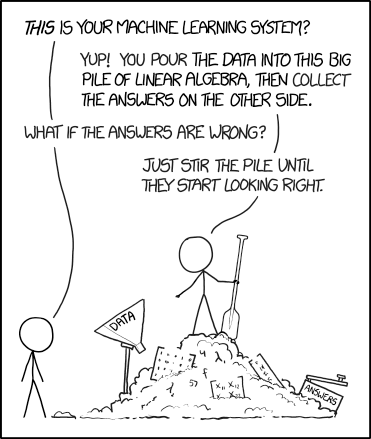
\includegraphics[scale=0.45]{figures/machine_learning}
\end{figure}
\end{frame}
%----------------------------------------------------------------------%
\subsection{Ejemplos para Motivarnos}
%----------------------------------------------------------------------%
\begin{frame}
\frametitle{Motivación}
\framesubtitle{La primera victoria y derrota de ML}

\begin{itemize}
  \item Contexto ?`similar? al de hoy: Epidemia de la gripe A en 2009
  \medskip
  \item En EEUU la forma de monitorear es a través de reportes de la CDC 
  \medskip
  \item La CDC agrega a nivel de ciudad, condado, estado, región y a nivel nacional
  \medskip
  \item Todo esto llevaba aproximadamente 10 días $\rightarrow$ demasiado tiempo para una epidemia
\end{itemize}
\end{frame}

%----------------------------------------------------------------------%

\begin{frame}
\frametitle{Motivación}
\framesubtitle{Google se ha unido a la conversación}

\begin{itemize}
  \item Google propuso un mecanismo ingenioso: {\bf Google Flu Trends}
  \bigskip
  \item Punto de partida: 
  \begin{itemize}
    \item Proporción de visitas semanales por Gripe A en hospitales 
    \item 9 regiones $\times$ 5 años (2003-2007) = $2,340$ datos
    \item Estos son los datos que tomaban 10 dias en elaborarse (comparemos con la Colombia de 2009)
  \end{itemize}
  \bigskip
  \item Google cruzó estos datos con las búsquedas sobre la gripe A
  \bigskip
  \item Con estos datos, construyeron un modelo para predecir intensidad de gripe A  
\end{itemize}  

\end{frame}

%----------------------------------------------------------------------%

\begin{frame}
\frametitle{Motivación}
\framesubtitle{Google se ha unido a la conversación}

\begin{itemize}
  \item ¿Un sólo modelo?
  \pause
  \bigskip
  \item Los investigadores de Google estimaron {\bf 450 millones} de modelos
  \bigskip
  \item Eligieron el que mejor predice sobe la intensidad de búsqueda
  \bigskip
  \item Les permite tener información diaria, semanal o mensual para cualquier punto de EEUU y el mundo
  \bigskip
  \item A Google le toma 1 día lo que a la CDC 10!
\end{itemize}  
\end{frame}
%----------------------------------------------------------------------%
\begin{frame}
\frametitle{Motivación}
\framesubtitle{Google se ha unido a la conversación}
\begin{figure}[H] \centering
            \captionsetup{justification=centering}  
            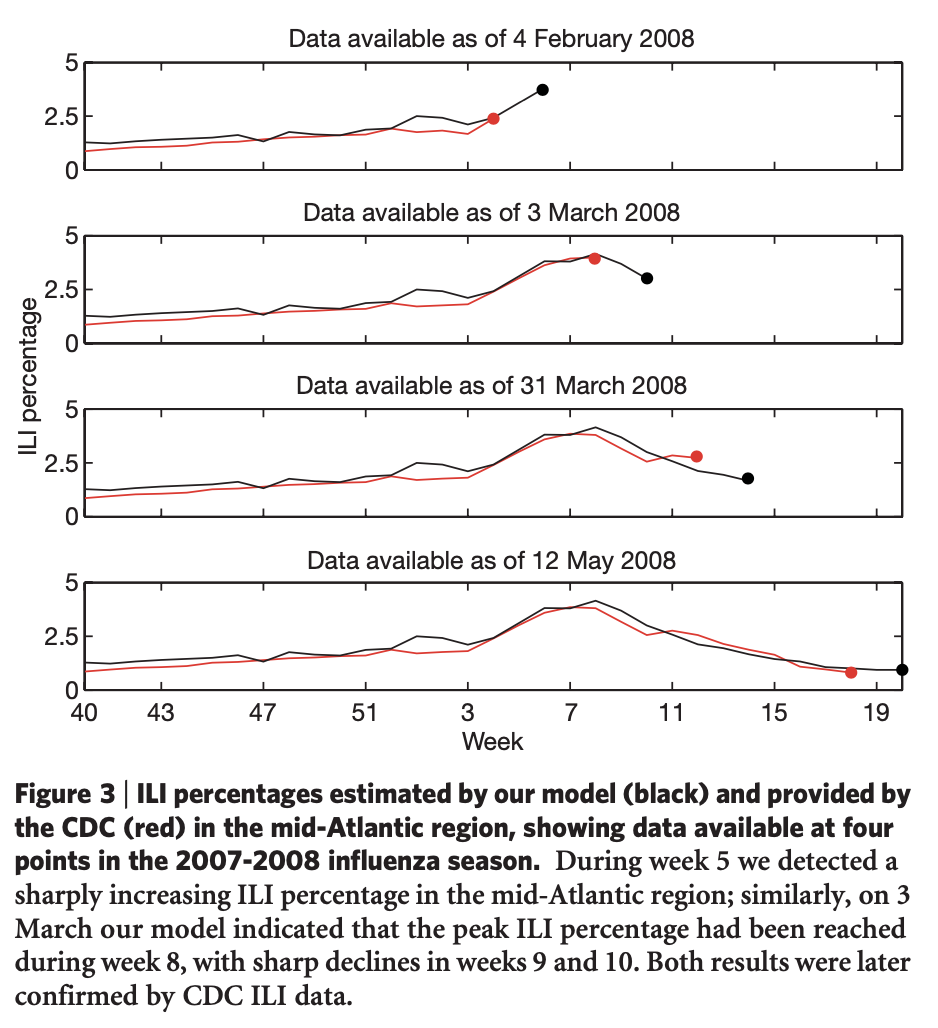
\includegraphics[scale=0.45]{figures/flu_trends}
    \end{figure}
\end{frame}


%----------------------------------------------------------------------%

\begin{frame}
\frametitle{Motivación}
\framesubtitle{El rey ha muerto, larga vida al rey}
  \begin{itemize}
    \item ¿Qué tienen en común Google Flu y Elvis?
    \bigskip
    \begin{itemize}
      \item Abanderados de la revolución
      \medskip
      \item Definió y redefinió las reglas sistemáticas para hallar la solución a un problema
      \medskip
      \item Éxito rotundo $\rightarrow$ Publicación en Nature! \url{https://www.nature.com/articles/nature07634}
      \medskip
      \item Pero como a Elvis el éxito fue efímero
      \medskip
      \item La predicciones comenzaron a sobre-estimar considerablemente la incidencia de la gripe A
      \medskip
      \item Google Flu esta ahora archivado (disponible al público)
      \medskip
      \item Continúa recolectando datos pero solo algunas instituciones científicas tienen accesso 
    \end{itemize}  
  \end{itemize}  
\end{frame}
%----------------------------------------------------------------------%

\begin{frame}
\frametitle{Motivación}

\begin{itemize}
      \item Otro ejemplo, los algoritmos de reconocimiento de cara: 
      \medskip
      \begin{itemize}
        \item no son reglas fijas basadas en que los humanos entendemos por rostros y a partir de ello buscar combinaciones de pixeles.
        \item son algoritmos que usan datos de fotos etiquetadas con un rostro y estiman una función $f(x)$ que predice si es un rostro o no a partir de pixeles x.
      \end{itemize}
      \medskip
      \item El aprendizaje de maquinas se hizo una realidad cuando los investigadores dejaron de afrontarlo de manera teórica y lo hicieron empíricamente.
      \medskip
      \item  Las similitudes con la econometría plantea interrogantes:
      \begin{itemize}
      \item  ¿Estos algoritmos están simplemente aplicando técnicas estándar a nuevos y grandes conjuntos de datos? 
      \item  Si hay herramientas empíricas fundamentalmente nuevas, ¿cómo encajan con lo que conocemos? 
      \item  Como economistas empíricos, ¿cómo podemos utilizarlas?
       \end{itemize}
\end{itemize}

\end{frame}



%----------------------------------------------------------------------%
\section{Sobre el curso}
%----------------------------------------------------------------------%
 \begin{frame}[noframenumbering]
\tableofcontents[currentsubsection]

\end{frame}
%----------------------------------------------------------------------%
\begin{frame}
\frametitle{Sobre el curso}


\begin{itemize}

  \item El aprendizaje automático en economía es muy nuevo y dinámico. 
  \medskip
  \item Estas 7 clases darán un {\it "snapshot"} de este campo en evolución.
  \medskip
  \item Estudiaremos ML a través de ejemplos, centrándonos en algunas aplicaciones y algoritmos de ML.
  \medskip
  \begin{itemize}
  \item Primera parte de la clase será teórica
  \medskip
  \item Break
  \medskip
  \item Segunda parte trabajo en \texttt{R}
  \end{itemize}
\end{itemize}

\end{frame}
 %----------------------------------------------------------------------%
\begin{frame}

\frametitle{Sobre el curso}
\begin{itemize}
  \medskip
  \item Un aspecto adicional de las clases es que intentaré resaltar cómo encaja el ML en (y dónde se diferencia de) los métodos cuantitativos existentes en la microeconomía aplicada.
  \medskip
  \item Lo que no haré es centrarme demasiado en los detalles de algoritmos y problemas computacionales.
  \medskip

\end{itemize}

\begin{quote}
The master-economist must possess a rare combination of gifts...He must be mathematician, historian, statesman, philosopher and \textcolor{andesred}{data scientist} – in some degree.
\end{quote}
\flushright{adaptado de {\it Keynes (1924), Economic Journal}}

\end{frame}
%----------------------------------------------------------------------%
\begin{frame}
\frametitle{Lecturas}


\begin{enumerate}


\item El libro de texto principal (nivel de maestría): James, Witten, Hastie and Tibshirani, An Introduction to Statistical Learning with Applications in R [ISLR] \href{https://www.statlearning.com/}{link}
\medskip
\item También es útil (nivel de primer año de doctorado): Hastie, Tibshirani, Friedman, Elementos de aprendizaje estadístico [ESL]. \href{https://web.stanford.edu/~hastie/ElemStatLearn/}{link} 
\medskip
\item Para los inquietos, estos artículos de introducción general en el Journal of Economic Perspectives estan muy interesantes:
  \begin{itemize}
    \item Varian (2014), “Big Data: New Tricks for Econometrics” \href{https://www.aeaweb.org/articles?id=10.1257/jep.28.2.3}{link}
    \item Mullainathan y Spiess (2017), “Machine Learning: An Applied Econometric Approach” \href{https://www.aeaweb.org/articles?id=10.1257/jep.31.2.87}{link}
  \end{itemize}
\medskip
\end{enumerate}


$\dots$ y otros que voy a mencionar en clase y los compartiremos en Slack
\end{frame}
%----------------------------------------------------------------------%
\section{Tipos de Aprendizaje}
%----------------------------------------------------------------------%
 \begin{frame}[noframenumbering]
\tableofcontents[currentsubsection]

\end{frame}
%----------------------------------------------------------------------%
\begin{frame}<1>[label=tipos_Aprendizaje]
\frametitle{Tipos de Aprendizaje}
\begin{itemize}


\item ML se divide en dos (¿?) ramas principales:
\medskip
  \begin{enumerate}

  \item Aprendizaje supervisado: Tenemos datos tanto sobre un resultado $y$ como sobre las variables explicativas $X$.
    \begin{itemize}
      \item Esto es lo más cercano al análisis de regresión que conocemos. De hecho, OLS es un  ejemplo de aprendizaje supervisado.
      \item Si $y$ es discreto, también podemos ver esto como un problema de clasificación.
      \item La mayoría de los ejemplos que veremos, y la mayor parte de nuestra discusión metodológica, caen en esta clase.
    \end{itemize}


  \pause
  \item  Aprendizaje no supervisado: No tenemos datos sobre $y$, solo sobre $X$.

  \begin{itemize}
    \item Queremos agrupar estos datos (sin especificar qué agrupar).
    \item Permite reducir la dimensionalidad y explorar datos
    \item Algunos algoritmos destacados: PCA, y  K-medias
  \end{itemize}

  \end{enumerate}
\end{itemize}
\end{frame}


%----------------------------------------------------------------------%
\begin{frame}
\frametitle{Tipos de Aprendizaje}


\begin{itemize}
  \item Aprendizaje supervisado
  \begin{itemize}
    \item para cada predictor $x_i$ hay una 'respuesta' observada $y_i$.
    \item lo que hacemos en econometría cae en esta rama
  \end{itemize}
\end{itemize}

\bigskip
\begin{figure}[H] \centering
  \captionsetup{justification=centering}

    \centering
    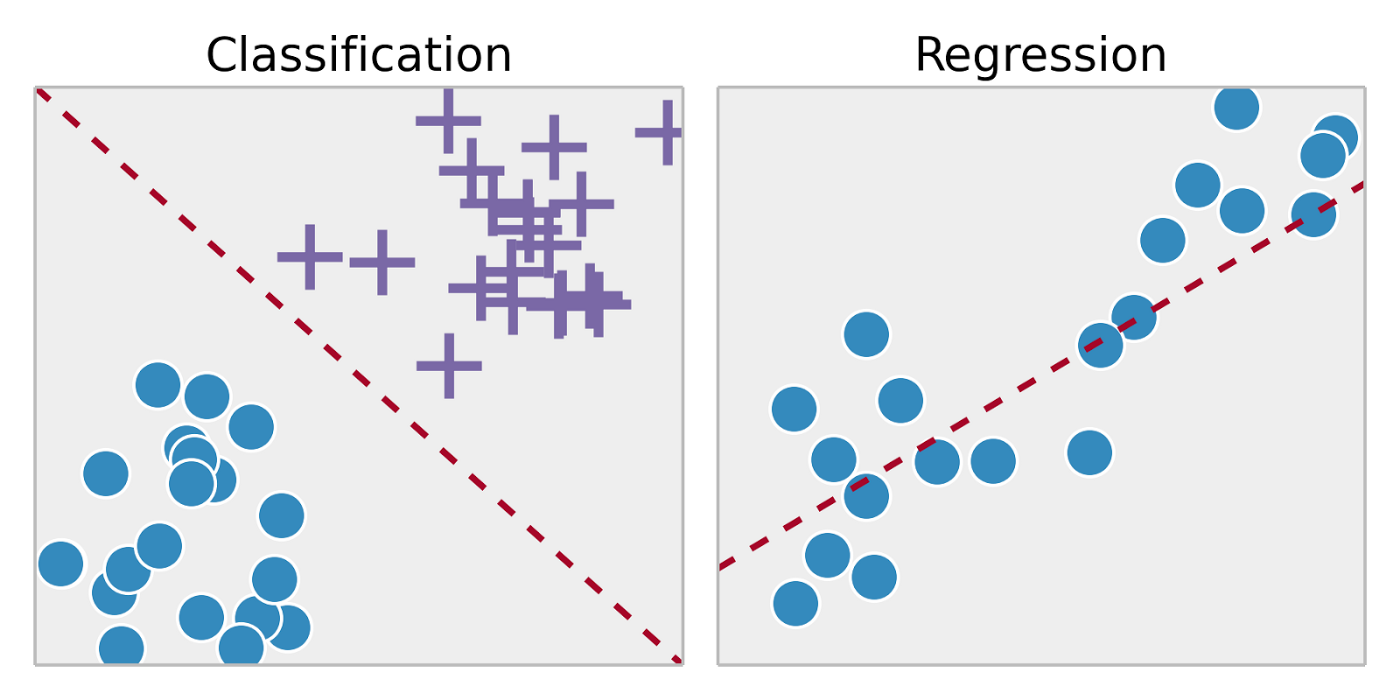
\includegraphics[scale=0.15]{figures/supevised}
  \\
  \tiny
  Source: \url{shorturl.at/opqKT}
  \end{figure}

\end{frame}

%----------------------------------------------------------------------%
%----------------------------------------------------------------------%
\againframe<2>{tipos_Aprendizaje}
%----------------------------------------------------------------------%
%----------------------------------------------------------------------%

\begin{frame}
\frametitle{Tipos de Aprendizaje}

\begin{itemize}
  \item  Aprendizaje no supervisado
  \begin{itemize}
    \item Observamos $X$ pero no las respuetas
    \item Ejemplo: agrupar datos
  \end{itemize}
  \end{itemize}

\bigskip
    \begin{figure}[H] \centering

    \centering
    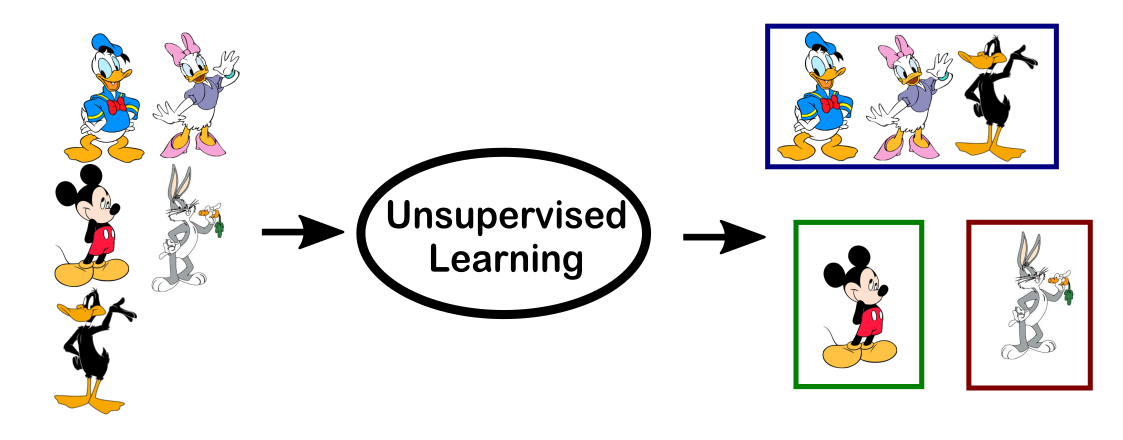
\includegraphics[scale=0.2]{figures/unsupevised}
  \\
  \tiny
  Source: \url{shorturl.at/opqKT}
\end{figure}


\end{frame}
%----------------------------------------------------------------------%
\section{A nadar}
%----------------------------------------------------------------------%
 \begin{frame}[noframenumbering]
\tableofcontents[currentsubsection]

\end{frame}
%----------------------------------------------------------------------%
\begin{frame}
\frametitle{Un modelo estadístico general}

\begin{itemize}
\item Asumamos que la relación entre la variable a predecir $y$ y los predictores $X$ esta dada por
\medskip
\begin{align}
Y=f(X)+u
\end{align}
\medskip
\item donde $f$ es una función fija pero desconocida de $X$, con $E(u)=0$ y $E(X'u)=0$
\medskip
\item $f$ no está restringida de ninguna manera; puede ser una función completamente arbitraria y compleja.
\end{itemize}


\end{frame}
%----------------------------------------------------------------------%
\begin{frame}
\frametitle{El paradigma clásico}


\begin{align}
Y=f(X)+u
\end{align}
\medskip
\begin{itemize}
  \item El interés esta en la inferencia
  \medskip
  \item Tests de hipótesis (std. err., tests)
  \medskip
  \item La $f(.)$ "correcta" nos ayuda a entender como $y$ es afectado por $X$
  \medskip
  \item Modelo: surge de la teoría
  
\end{itemize}

\end{frame}

%----------------------------------------------------------------------%

\begin{frame}
\frametitle{El paradigma predictivo}



\begin{align}
Y=f(X)+u
\end{align}

\begin{itemize}
  \item El objetivo del aprendizaje supervisado es predecir $y$ basada en las características $X$.
  \medskip
  
  
  \item Debido a que nos ayuda a hacer una predicción, es útil estimar $f(.)$
  \medskip
  \item Entonces la  $f(.)$ ``correcta'' es la que es capaz de predecir (no hacer inferencia!)
  \medskip
  \item Modelo?
  \pause
  \item Como en predicción {\bf no} nos interesa $f(.)$ en si misma, podemos tratarla como una {\it black box}, cualquier aproximación que nos da una buena predicción funciona. Recordemos:

\pause
  \begin{quote}
  \centering
  \bf ``Lo que sea que funciona, funciona...''
  \end{quote}
\end{itemize}



\end{frame}

%----------------------------------------------------------------------%

\begin{frame}
\frametitle{El paradigma predictivo}

\begin{itemize}

  \item A lo largo del curso vamos a explorar varios algoritmos lineales y no lineales que nos permitan estimar $f(.)$
  \medskip
  \item Estos métodos podemos resumirlos  en dos grandes ramas
  \medskip
  \begin{enumerate}
    \item Modelos paramétricos
    \medskip
    \item Modelos no paramétricos
  \end{enumerate}

\end{itemize}


\end{frame}


%----------------------------------------------------------------------%

\begin{frame}
\frametitle{Como estimamos $f(.)$?}
\framesubtitle{Métodos paramétricos}


\begin{itemize}
 \item Supongamos que tenemos los siguientes datos 
\end{itemize}

\begin{figure}[H] \centering
  \centering
  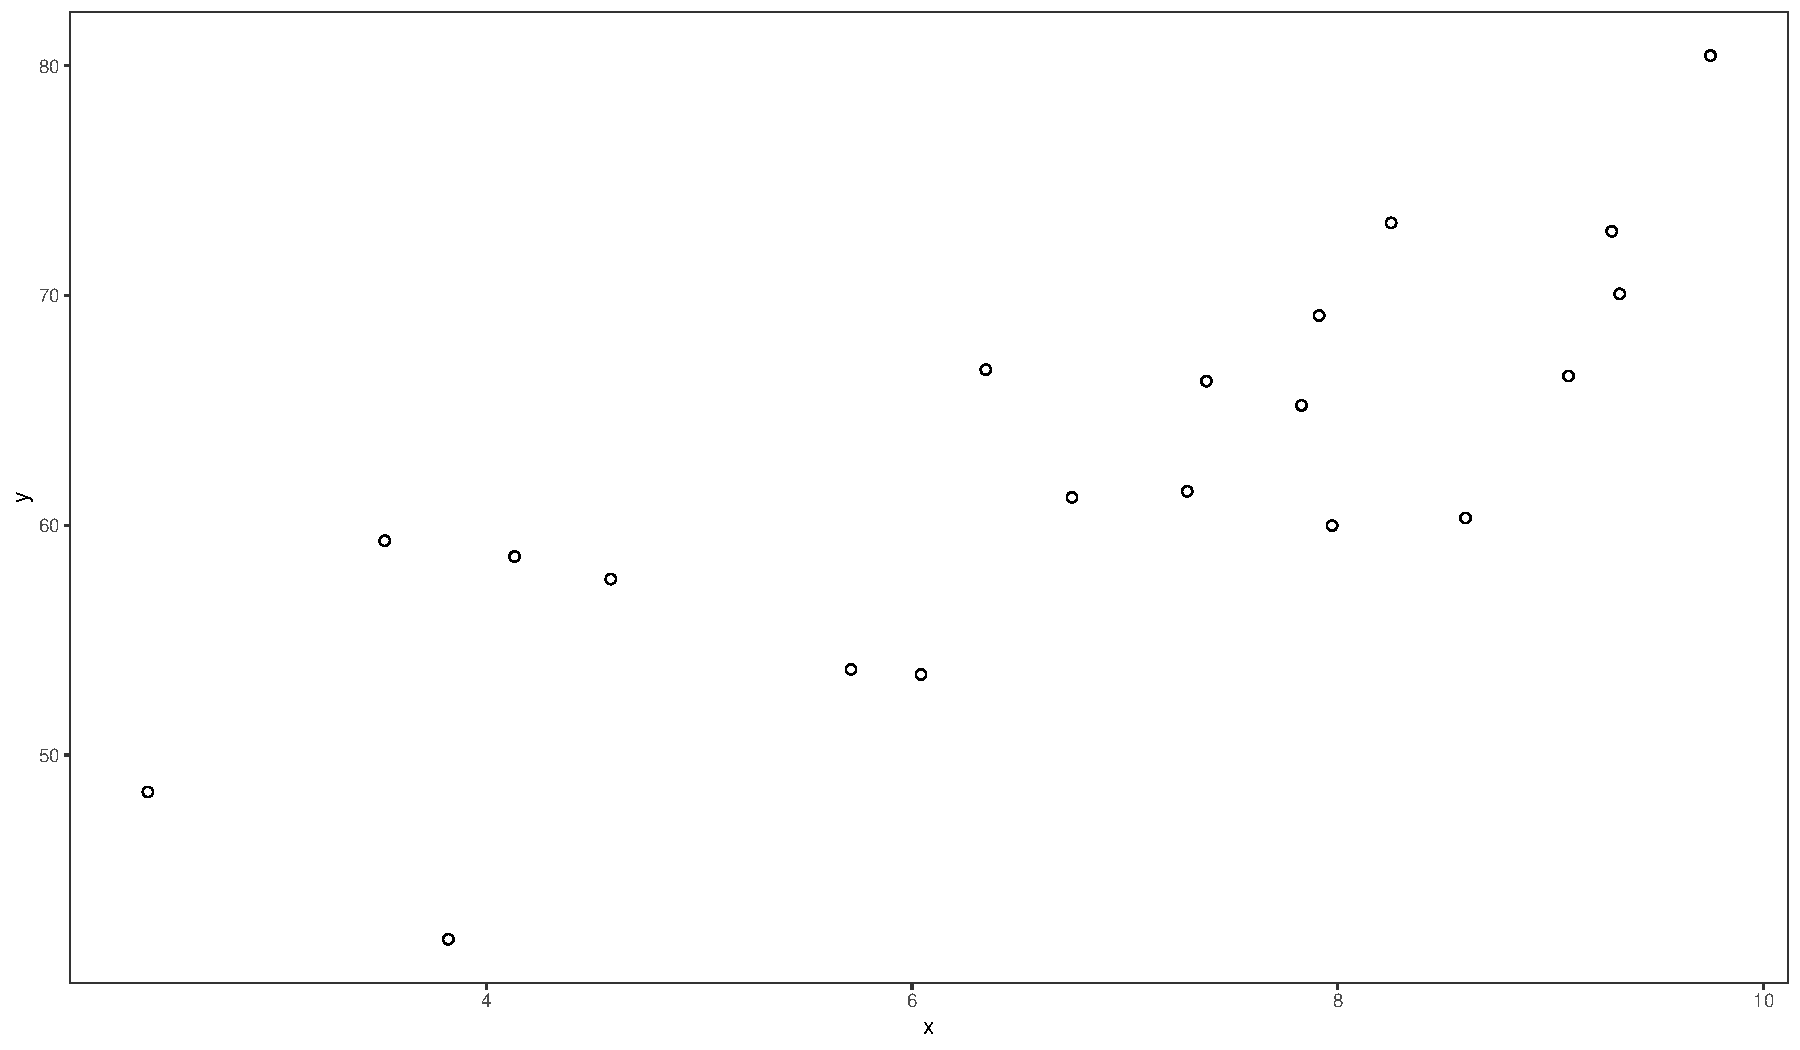
\includegraphics[scale=0.25]{figures/fig_1.pdf}
  \\
  \tiny
  Fuente: datos simulados
\end{figure}

\end{frame}

%----------------------------------------------------------------------%

\begin{frame}
\frametitle{Como estimamos $f(.)$?}
\framesubtitle{Métodos paramétricos}

\begin{itemize}
  \item Los modelos paramétricos generalmente envuelven un enfoque de 2 pasos:
  \medskip

  \begin{enumerate}
    \item Primero hacemos un supuesto sobre la forma funcional de $f(.)$. La mas común es que es lineal en $X$
    \begin{align}
    f(X) = \beta_0 + \beta_1 X_1 + \dots + \beta_p X_p 
    \end{align}

    \item Luego de seleccionar el modelo, necesitamos un procedimiento que nos ayude a "ajustar" o "entrenar" el modelo
  \end{enumerate}
  \medskip

  \item Este enfoque se conoce como paramétrico porque reduce el problema de estimar $f(.)$ a estimar un conjunto de parámetros
\end{itemize}

\end{frame}

%----------------------------------------------------------------------%

\begin{frame}
\frametitle{Como estimamos $f(.)$?}
\framesubtitle{Métodos paramétricos}

\begin{align}
   f(X) = \beta_0 + \beta_1 X_1 + \dots + \beta_p X_p 
\end{align}

\begin{figure}[H] \centering
  \centering
  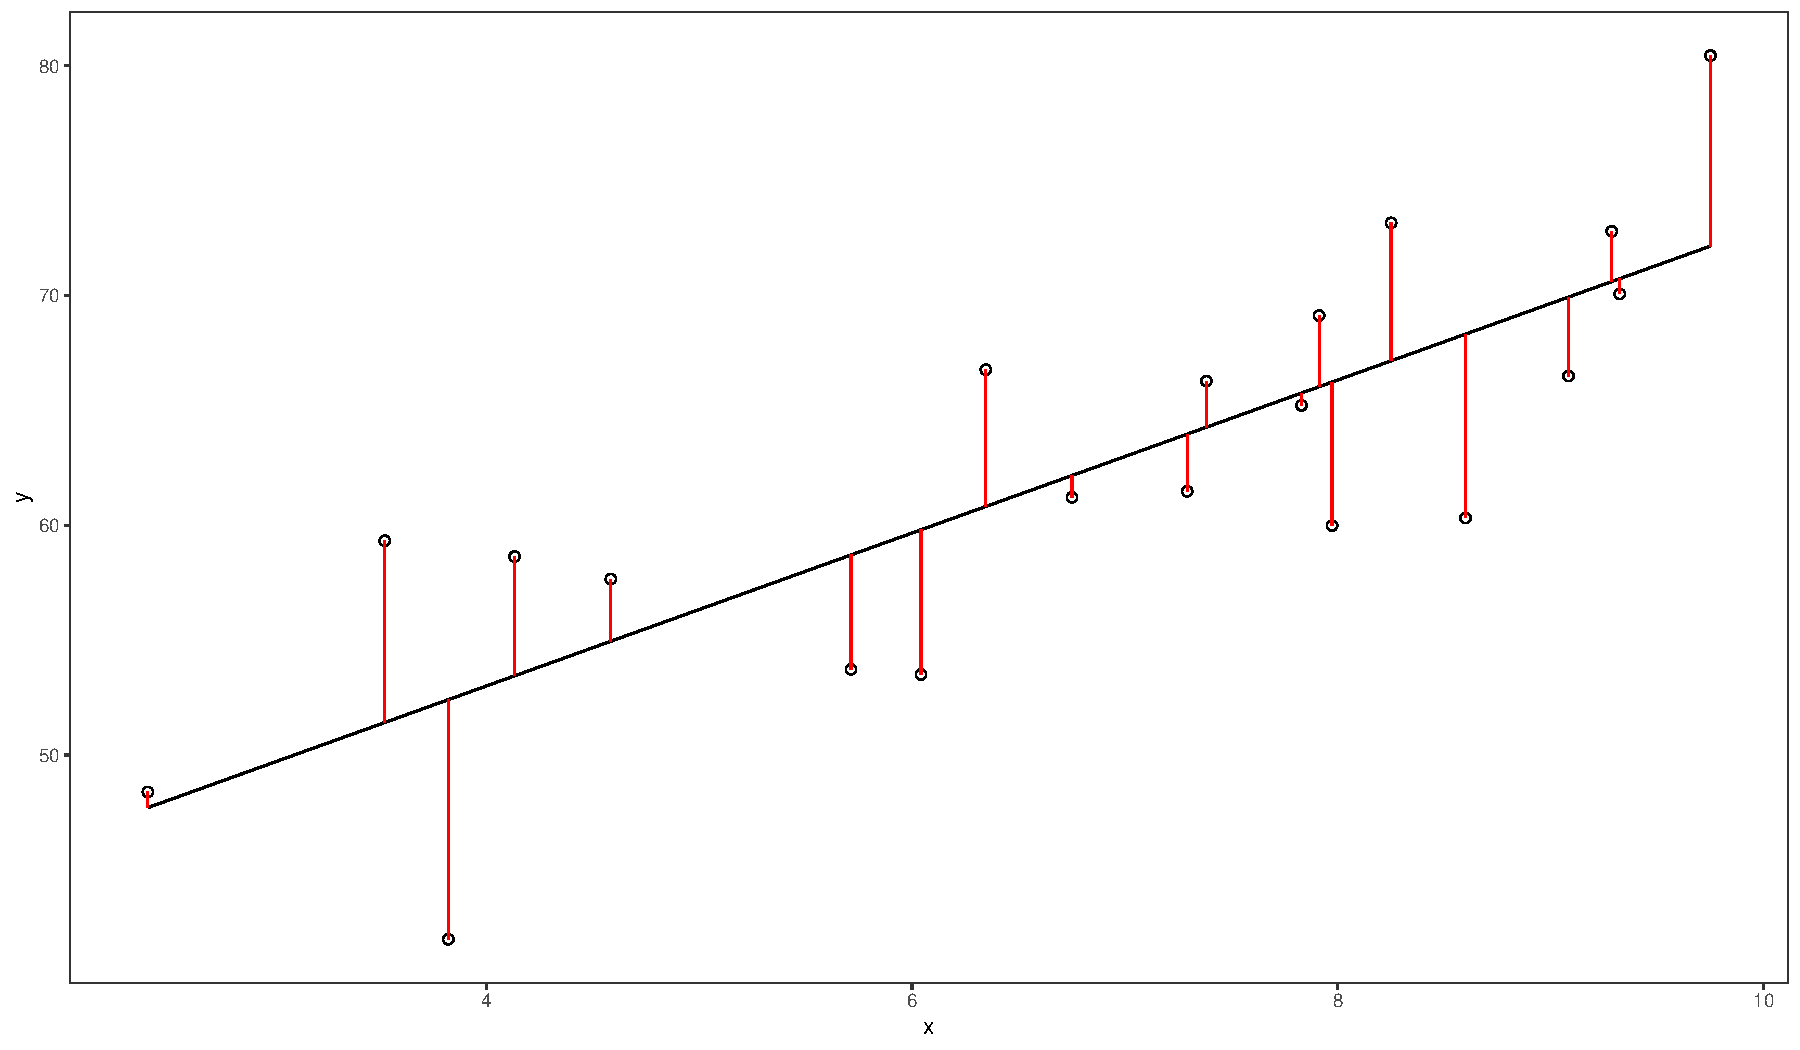
\includegraphics[scale=0.2]{figures/fig_1b.pdf}
  \\
  \tiny
  Fuente: datos simulados
\end{figure}

\end{frame}
%----------------------------------------------------------------------%

\begin{frame}
\frametitle{Como estimamos $f(.)$?}
\framesubtitle{Métodos no paramétricos}
\begin{itemize}
\item No hacen supuestos explícitos sobre la forma funcional de $f(.)$
\medskip
\item Buscan estimar $f(.)$ que se acerque lo mas posible a los puntos sin ser lo demasiada rígida u ondulada
\medskip
\item Tienen la ventaja que se pueden adaptar a mas formas posibles de $f(.)$
\medskip
PEro suelen necesitar un número mas alto de observaciones y en algunos casos ser poco robustos.
\end{itemize}

\end{frame}
%----------------------------------------------------------------------%

\begin{frame}
\frametitle{Como estimamos $f(.)$?}
\framesubtitle{Métodos no paramétricos}

\begin{align}
  f(X)=g(X) \text{donde g es un spline}
\end{align}

\begin{figure}[H] \centering
  \centering
  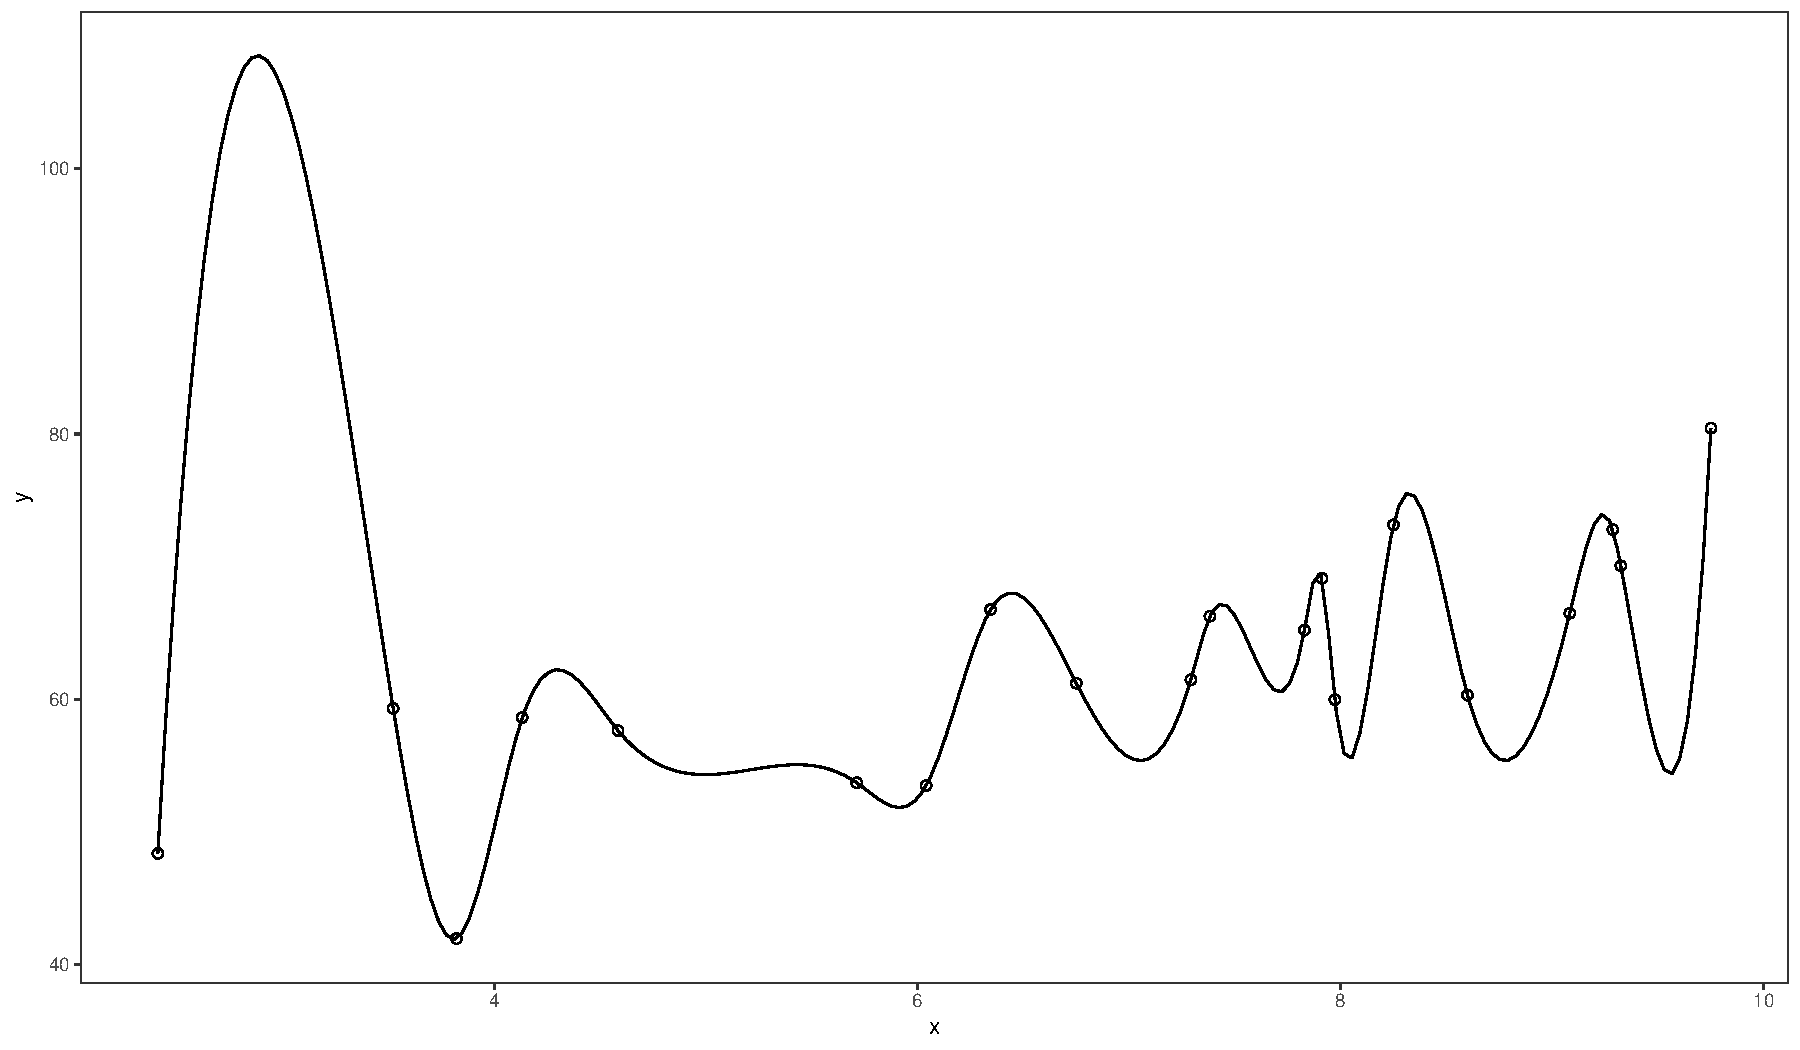
\includegraphics[scale=0.2]{figures/fig_1c.pdf}
  \\
  \tiny
 Fuente: datos simulados
\end{figure}

\end{frame}
%----------------------------------------------------------------------%
\subsection{Regresión Lineal}
%----------------------------------------------------------------------%
 \begin{frame}[noframenumbering]
\tableofcontents[currentsubsection]

\end{frame}
%----------------------------------------------------------------------%
\begin{frame}
\frametitle{Regresión Lineal}

\begin{figure}[H] \centering
  \centering
  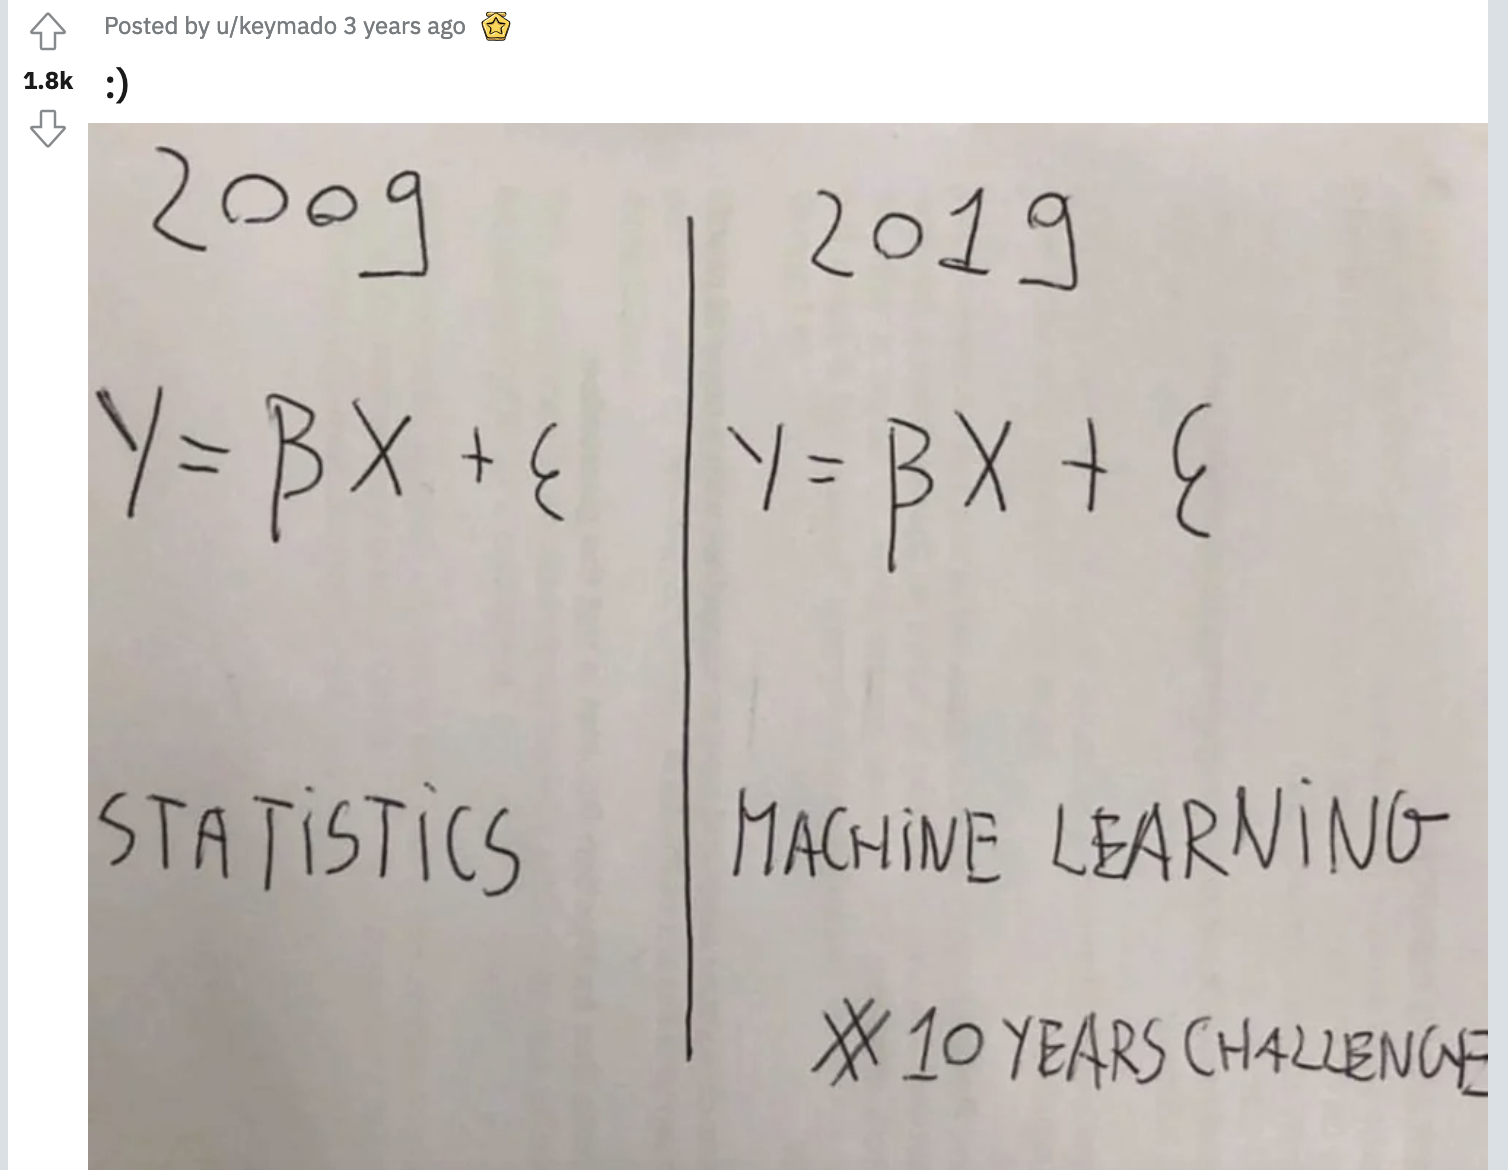
\includegraphics[scale=0.25]{figures/ten_years.png}
  \\
  \tiny
  Fuente: \url{https://www.reddit.com/r/datascience/comments/ah0q69/_/}
\end{figure}

\end{frame}
%----------------------------------------------------------------------%
\begin{frame}
\frametitle{Regresión Lineal}

\begin{itemize}


\item El problema es:
\begin{align}
y=f(X)+u
\end{align}

\item proponemos que:
\begin{align}
  f(X) = \beta_0 + \beta_1 X_1 + \dots + \beta_p X_p 
\end{align}

\item El problema se reduce a encontrar los $\beta$s

\begin{itemize}
  \footnotesize
  \item Method de Momentos 
  \item MLE 
  \item OLS: minimiza SSR ($e'e$) 
  \begin{itemize}
    \tiny
  \item donde $e=y-\hat y=y-X\hat\beta$
  \end{itemize}  
\end{itemize}



\end{itemize}
\end{frame}


%----------------------------------------------------------------------%
\subsection{Precisión del modelo}
%----------------------------------------------------------------------%
\begin{frame}
\frametitle{Como medimos: ``Lo que sea que funciona, funciona...''}

\begin{itemize}
  \item Con los parámetros podemos entonces recobrar la predicción
    \begin{align}
      \hat{y} &= \hat{f}(X) \\
              &= \hat{\beta}_0 + \hat{\beta}_1 X_1 + \dots + \hat{\beta}_p X_p  
    \end{align}
\item Como sabemos que funcionó bien?
\pause
\item En estos problemas la medida más utilizada  es el {\it error cuadrático medio (MSE)} 
\begin{align}
MSE &= \frac{1}{n} \sum_{i=1}^n (y_i - \hat{f}(X) )^2
\end{align}
\end{itemize}


\end{frame}
%----------------------------------------------------------------------%
\begin{frame}
\frametitle{Como medimos: ``Lo que sea que funciona, funciona...''}
\begin{itemize}
  \item Notemos que esto no es otra cosa que la suma de los residuales al cuadrado
  \begin{align}
  MSE &= \frac{1}{n} \sum_{i=1}^n (y_i - \hat{f}(X) )^2 \\ 
      &= \frac{1}{n} \sum_{i=1}^n (y_i - \hat{y} )^2 \\ 
      &= \frac{1}{n} \sum_{i=1}^n (e)^2 \\ 
      &= RSS
  \end{align}
  \item Esta medida nos da una idea de {\it lack of fit} que tan mal ajusta el modelo a los datos
\end{itemize}

\end{frame}
%----------------------------------------------------------------------%
\begin{frame}
\frametitle{Como medimos: ``Lo que sea que funciona, funciona...''}

\begin{itemize}
\item Un problema del RSS es que nos da una medida absoluta de ajuste de los datos, y por lo tanto no esta claro que constituye un buen RSS.
\medskip
\item Una alternativa muy usada en economía es el $R^2$
\medskip
\item Este es una proporción (la proporción de varianza explicada), 
\begin{itemize}
  \item toma valores entre 0 y 1,
  \item   es independiente de la escala (o unidades) de $y$
 \end{itemize} 
\medskip
\begin{align}
R^2 &= 1 - \frac{\sum_{i=1}^n (y_i - \hat{y} )^2 }{\sum_{i=1}^n (y_i - \bar{y} )^2 }  \\
    &= 1 - \frac{RSS}{TSS} 
\end{align}
\end{itemize}

\end{frame}
%----------------------------------------------------------------------%
\section{Recap}
%----------------------------------------------------------------------%
\begin{frame}[noframenumbering]
\tableofcontents[currentsubsection]

\end{frame}
%----------------------------------------------------------------------%
\begin{frame}
\frametitle{Quick Recap antes de ir a \texttt{R}}

\begin{itemize}
  \item Vamos a ver distintos algoritmos donde el objetivo es predecir bien
  \medskip
  \item {\it ``Lo que sea que funciona, funciona...''}
  \medskip
  \item La medida más utilizada en problemas de regresión es el MSE

\end{itemize}

\end{frame}
%----------------------------------------------------------------------%
\section{Break}
\begin{frame}
\frametitle{}

\begin{centering}
\huge
\textcolor{andesred}{Volvemos en 15 mins con \texttt{R} }

\end{centering}

\end{frame}
%----------------------------------------------------------------------%
\section{\texttt{R para ML}}
%----------------------------------------------------------------------%
\begin{frame}
\frametitle{R para ML}

\begin{figure}[H] \centering
  \centering
  
\includegraphics[scale=0.35]{figures/baticomputer_meme.jpg}
  \\
  \tiny photo from \url{https://www.dailydot.com/parsec/batman-1966-labels-tumblr-twitter-vine/}
\end{figure}

\end{frame}
%----------------------------------------------------------------------%
%----------------------------------------------------------------------%
\end{document}
